\documentclass[12pt]{report}

\usepackage{amsmath,amssymb,amsthm,bm,caption,enumitem,float,geometry,graphicx}
\usepackage{hyperref,mathrsfs,titlesec,tikz,tkz-euclide,wrapfig}

\usepackage[math]{cellspace}
\geometry{a4paper, margin=1in}

\hypersetup{hidelinks}
%\hyphenpenalty=10000

\title{Projective Geometry}
\author{Tejaswi K, Niti Torphe, Ruchith R, Saroj Kumar \and Supervisor: Dr. Steven Spallone}
\date{}

\titleformat{\chapter}
    [frame]
    {\bfseries\Huge}
    {\Large CHAPTER \thechapter}
    {1ex}{\centering}[]

\DeclareCaptionFormat{capfmt}{\textbf{#1 #2}#3}
\captionsetup{format=capfmt}

\newtheorem{theorem}{Theorem}
\newtheorem{prop}{Proposition}
\newtheorem{lemma}{Lemma}

\theoremstyle{definition}
\newtheorem{definition}{Definition}
\newtheorem*{ex}{Ex}

\theoremstyle{remark}
\newtheorem*{notation}{Notation}
\newtheorem*{remark}{Remark}

\newcommand\conop{\oplus_{\vphantom{\dfrac{}{}}O}}
\newcommand\tgrp[3]{\mathrm{#1}_{#2}(\mathbb{#3})}
\newcommand\SO[2]{\tgrp{SO}{#1}{#2}}
\newcommand\AffF[2]{\mathbb{A}^{#1}(\mathbb{#2})}
\newcommand\Aff[1]{\mathbb{A}^{#1}}
\newcommand\norm[1]{\left\lVert{#1}\right\rVert}

\newcommand{\R}{\mathbb{R}}
\newcommand{\Q}{\mathbb{Q}}
\newcommand{\Z}{\mathbb{Z}}
\newcommand{\C}{\mathbb{C}}
\newcommand{\N}{\mathbb{N}}
\newcommand{\F}{\mathbb{F}}
\newcommand{\Ps}{\mathbb{P}}

\renewcommand\qedsymbol{$\blacksquare$}

\DeclareMathOperator{\A}{A}
\DeclareMathOperator{\GA}{GA}
\DeclareMathOperator{\GL}{GL}
\DeclareMathOperator{\Hom}{Hom}
\DeclareMathOperator{\End}{End}
\DeclareMathOperator{\Prj}{P}
\DeclareMathOperator{\ch}{ch}

\setlength{\cellspacetoplimit}{5pt}
\setlength{\cellspacebottomlimit}{5pt}

\addtocontents{toc}{\protect\setcounter{tocdepth}{1}}

%% tejaswi
%%
%%\documentclass[a4paper,12pt]{report}
%%\usepackage{amsmath,amsthm,amssymb,graphicx,float,tikz,tkz-euclide,geometry,hyperref}
%%
%%\hypersetup{hidelinks}
%%
%%\hyphenpenalty=10000
%%
%%\newtheorem*{theorem}{Theorem}
%%\newtheorem*{prop}{Proposition}
%%\newtheorem*{lemma}{Lemma}
%%
%%\theoremstyle{definition}
%%\newtheorem*{definition}{Definition}
%%\newtheorem*{ex}{Ex}
%%
%%\theoremstyle{remark}
%%\newtheorem*{remark}{Remark}
%%
%%\renewcommand\qedsymbol{$\blacksquare$}
%%
%%\newcommand{\R}{\mathbb{R}}
%%\newcommand{\Q}{\mathbb{Q}}
%%\newcommand{\Z}{\mathbb{Z}}
%%\newcommand{\C}{\mathbb{C}}
%%\newcommand{\N}{\mathbb{N}}
%%\newcommand{\F}{\mathbb{F}}
%%
%%\addtocontents{toc}{\protect\setcounter{tocdepth}{1}}


\begin{document}
\maketitle

\chapter{Axiomatic Approach}

\section{First Axiom}

\begin{definition}
    A plane is a triple $(\pt,\li,\ic).$ The set $\pt$ consists of the points, the set $\li$ consists of the lines, and the inclusion $\ic \subseteq \pt \times \li$ is an incidence relation. 
\end{definition}

\begin{definition}
    If $l,m \in \li$ such that either $l = m$ or for every $P \in \pt,$ $(P,l),(P,m) \not \in \ic,$ then we call $l$ and $m$ are parallel.
\end{definition}

\begin{axiom}[1]
    For any $P,Q \in \pt,$ there exists a unique $l \in \li$ such that $P \ic l$ and $Q \ic l.$ We write $l=P+Q.$
\end{axiom}

For any given $l,m \in \li$, if there exists a unique $P \in \pt$ such that $(P,l),(P,m) \in \ic,$ then $l \nparallel m$. If there exists more than one point, without loss of generality, assume $P \ic l,$ $Q \ic l,$ $P \ic m,$ and $Q \ic m,$ by axiom 1, $l=m,$ hence $l \parallel m.$

Let $\pt_l \subset \pt$ be the set of all points on $l$ that is $\pt_l := \{ P \in \pt \: | \: (P,l) \in \ic\}.$

\section{Second Axiom}

\begin{axiom}[2]
    For any $P \in \pt$ and $l \in \li,$ there exists a unique $m \in \li$ such that $P \ic m,$ and $l \parallel m.$
\end{axiom}

\begin{theorem}
    Parallel is an equivalence relation.
\end{theorem}
\begin{proof}
    For any $l \in \li$, $l=l$, hence $l \parallel l.$ If $l,m \in \li$ and $l \parallel m,$ then $m \parallel l.$ Assume $l \parallel m,$ and $m \parallel n$. If there exists no $P \in \pt$ such that $(P,l),(P,n) \in \ic,$ then $l \parallel n.$ If there exists a $P \in \pt$ such that $(P,l),(P,n) \in \ic,$ then by axiom 2, there exists a unique $r \in \li$ such that $P \ic r,$ and $ r \parallel m.$ Hence, $l=n$ and $l \parallel n.$
\end{proof}

An equivalence class of parallel line is called a pencil of parallel lines.

\begin{theorem}
    Suppose that there exist three distinct pencils $\pi_1, \pi_2$ and $\pi_3$ of parallel lines. Then any pencil $\pi$ contains as many lines as the number of points on any line.
\end{theorem}
\begin{proof}
    Let $l \in \pi_1$, $m \in \pi_2.$ For every $Q_i \in \pt$ such that $Q_i \ic l,$ by axiom 2, there exists exactly one $m_i \in \li$ such that $m \nparallel m_i.$ If $m_i = m_j,$ by axiom 1, $P_i=P_j$ and therefore $i=j.$ \\
    For every $l_i \in \pi_2$, as $l \parallel l_i,$ there exists exactly one $P_i \in \pt$ such that $P_i \ic l$ and $P_i \ic l_i$. If $P_i = P_j$ and since $l_i \parallel l_j,$ by definition, $l_i=l_j$ and therefore $i=j.$  \\
    We found a one-to-one correspondence between the points on $l$ and the lines in $\pi_2.$ Hence, for given two distinct pencils, the number of lines in one pencil is equal to the number of points on a line in another pencil. Now, we use the fact that we have 3 distinct pencils of parallel lines. The number of points on a line in $\pi_3$ is equal to the number of lines in $\pi_1$ and the number of points on a line in $\pi_3$ is equal to the number of lines in $\pi_2,$ hence the number of lines in $\pi_1$ and $\pi_2$ is equal and therefore the number of points on any line in $\pi_1, \pi_2$ and $\pi_3$ is equal.
\end{proof}

\section{Third Axiom}
\begin{axiom}[3]
    There exist three distinct points $A,B,C \in \pt$ such that $(C,A+B) \notin \ic$ We also say that there exist three non-collinear points.
\end{axiom}

The smallest structure possible with this geometry is $\Z_2^2.$

\section{Fourth Axiom}
\begin{definition}
    A map $\sigma: \pt \mapsto \pt$ is called a dilatation if, for any $P,Q \in \pt$ such that $P \neq Q$ and their images $P'$ and $Q'$ are given. If $l' \in \li$ such that $l' \parallel P+Q$ and $P' \ic l'$, then $Q' \ic l'.$
\end{definition}

We can give two examples,
\begin{itemize}
    \item For every $P \in \pt$ and given $P' \in \pt,$ $P^{\sigma}=P'$
    \item For every $P \in \pt,$ $P^{\sigma}=P$
\end{itemize}

\begin{theorem}
    A dilatation $\sigma$ is uniquely determined by the images $P', Q'$ of two distinct points $P$ and $Q$. If $P'=Q',$ then $\sigma$ is degenerate and all points are mapped to $P'$ and if $P' \neq Q',$ then $\sigma$ is one-to-one and onto a map.
\end{theorem}
\begin{proof}
    For $R \notin \pt_{P+Q},$ then $R+P \nparallel R+Q.$ Let $l' \in \li$ such that $P' \ic l'$ and $l' \parallel R+P,$ by definition, $R' \ic l'.$ Let $l'' \in \li$ such that $Q' \ic l''$ and $l'' \parallel Q+P,$ by definition, $R' \ic l''.$ Hence, $l' \nparallel l'',$ and there exists a unique point $R'$ such that $(R',l'),(R',l'') \in \ic.$ Therefore, $R'$ is uniquely determined. \\
    For $R \in \pt_{P+Q},$ such that $P \neq R.$ By axiom 3, there exists a $S \notin \pt_{P+Q}$. If the point $R \in \pt_{P+S},$ since $P,R \in \pt_{P+Q},$ and $P,R \in \pt_{P+S},$ then $P+Q=P+S.$ Therefore suppose $R \notin \pt_{P+S}$ and we uniquely determine $S'$ using the images $Q'$ and $P',$ and later uniquely determine $R'$ using the images $S'$ and $P'.$ \\
    Suppose $P' = Q',$ the degenerate map $\gamma,$ which maps every point to $P'$ has the same effect as $\sigma$ which sends both $P$ and $Q$ to $P'$. Hence by uniqueness, $\sigma = \gamma.$ \\
    Suppose $P' \neq Q',$ and let $R'$ be a given point. For $R' \notin \pt_{P'+Q'},$ then $R'+P' \nparallel R'+Q'.$ Let $l_1 \in \li$ such that $P \ic l_1$ and $l_1 \parallel R'+P'$ and let $l_2 \in \li$ such that $Q \ic l_2$ and $l_2 \parallel Q'+P'.$ Then $l_1 \nparallel l_2,$ and hence there exists a unique point $R$ such that $(R,l_1),(R,l_2) \in \ic.$ Therefore, $R$ is uniquely determined.  Suppose $R \in \pt_{P+Q},$ then $P \ic l_1$ and $Q \ic l_2,$ hence $P+Q = l_1$ or $P+Q = l_2.$ By definition, $P'+Q' \parallel P' + R'$ or $P'+Q' \parallel Q' + R'$, which contradicts. Hence, with the help of given images of $P$ and $Q$ and using the point we found ($R$). We conclude that $R'$ is the image of $R.$ For $R' \in \pt_{P'+Q'},$ such that $P \neq R.$ According to axiom 3, there exists a $S' \notin \pt_{P'+Q'}$. If the point $R' \in \pt_{P'+S'},$ since $P',R' \in \pt_{P'+Q'},$ and $P',R' \in \pt_{P'+S'},$ then $P'+Q'=P'+S'.$ Therefore suppose $R' \notin \pt_{P'+S''}$ and we uniquely determine $S$ whose image is $S'.$ and proof that we can uniquely find $R$ whose image is $R'$ using the images $P'$ and $Q'.$
\end{proof}
\begin{definition}
    Let $\sigma$ be a non-degenerate dilatation and $P \in \pt.$ For any $l \in \li$ such that $P \ic l$ and $\sigma P \ic l$ is called a trace of $P.$ If $P = \sigma P,$ then all the lines passing through $P$ is the trace of $P.$ If $P \neq \sigma P,$ then the trace of $P$ is unique and $=P+Q.$ Let the set of traces of the non-singular dilatation be $\zeta_\sigma.$
\end{definition}
\begin{theorem}
    Let $\sigma$ be a non-degenerate dilation, $P \in \pt$ and $l$ be a trace of $P.$ If $Q$ lies on $l,$ then $\sigma Q$ also lies on $l$. 
\end{theorem}
\begin{proof}
    Assume $Q \neq P,$ therefore $l=P+Q.$ Let $\sigma P$ and $\sigma Q$ be the images of $P$ and $Q$, respectively. Then $\sigma Q \neq \sigma P,$ and, by definition, $\sigma P + \sigma Q \parallel l.$ But $\sigma P\ic \sigma P+ \sigma Q$ and $ \sigma P \ic l,$ hence $l=\sigma P+ \sigma Q.$ Therefore $\sigma Q$ lies on $l.$
\end{proof}
\begin{coro}
    The intersection of non-parallel traces is a fixed point.
\end{coro}
This concludes us with three possibilities for the traces of non-singular dilatation, which are:
\begin{itemize}
    \item $\sigma=1,$ if and only if $\zeta_\sigma = \li$
    \item if $\sigma \neq 1$ and if $P$ is a fixed point of $\sigma,$ then $\zeta_\sigma := \{ l=P+Q \; | \;Q \in \pt\}$ 
    \item if $\sigma$ fixes no point, then $\zeta_\sigma = \pi,$ where $\pi$ is some pencil of parallel lines
\end{itemize}

\begin{definition}
    A non-singular dilatation $\tau$ is called a translation if either $\tau = 1$ or $\tau$ has no fixed point. If $\tau \neq 1,$ then traces of $\tau$ form a pencil $\pi$ of parallel lines which is called the direction of $\tau.$
\end{definition}

\begin{theorem}
    A translation $\tau$ is uniquely determined by the image $P'$ of one point $P.$
\end{theorem}

\begin{proof}
    Let $l \in \zeta_\tau$ such that $P \ic l.$ For $Q \not \in \pt_l,$ let $l' \parallel l,$ and $Q \ic l$ then $l' \in \zeta_\tau$ and $\tau Q \ic l.$  Let $m,m' \in \li$ such that $m=P+Q, \; P' \ic m', \: m' \parallel m.$ Then by definition, $ \tau Q \ic m'.$ Since $l \not \parallel m,$ hence $l' \not \parallel m'$. Since $\tau Q \ic m'$ and $\tau Q \ic l',$ therefore $\tau Q$ is uniquely determined. \\
    For $Q \in \pt_l,$ and $Q \neq P,$ by axiom 3, there exists a $S \notin \pt_{l}$. let $l'' \parallel l,$ and $S \ic l$ then $l'' \in \zeta_\tau$ and $\tau S \ic l.$  Let $n,n' \in \li$ such that $n=P+S, \; P' \ic n', \: n' \parallel n.$ Then by definition, $ \tau S \ic m'.$ Since $l \not \parallel n,$ hence $l' \not \parallel n'$. Since $\tau S \ic m'$ and $\tau S \ic l',$ therefore $\tau S$ is uniquely determined and using the image of $S,$ we can uniquely determine the image of $Q$. 
\end{proof}

\begin{theorem}
    Dilatations form a group $D$ and translations form an invariant subgroup $T$ of $D$. If $\sigma$ is a dilatation and $\tau \neq 1,$ a translation. then $\tau$ and $\sigma \tau \sigma^{-1}$ have the same direction.
\end{theorem}
\begin{proof}
    Let $\sigma_1, \sigma_2$ be two dilatations. 
    \[ P+Q \parallel \sigma_2 P + \sigma_2 Q \parallel \sigma_1 \sigma_2 P+ \sigma_1 \sigma_2 Q \]
    Since dilatations are one-one and onto, we can always define an inverse map and let it be $\sigma^{-1}$. 
    \[ \sigma^{-1}P+\sigma^{-1}Q \parallel \sigma\sigma^{-1}P+\sigma\sigma^{-1}Q = P+Q \]
    Hence, we show $\sigma^{-1}$ is a dilatation.
    We satisfy all the conditions to show that dilatations form a group.

    Let $\tau$ be a translation. Suppose $\tau^{-1}$ fixes a point $P$, $\tau^{-1}P=P,$ and hence, $P=\tau P.$ Therefore, $\tau = 1,$ $\tau_{-1}=1. $ This proves that inverse of a translation is a translation. \\
    Let $\tau_1, \tau_2$ be two translations. Suppose $\tau_1 \tau_2$ fixes a point.     \[ \tau_1 \tau_2 P=P \: \Rightarrow \tau_2 P= \tau_1^{-1}P \]   \[ \therefore \tau_1^{-1} =\tau_2 \: \Rightarrow \tau_1 \tau_2=1 \]
    We satisfy all the conditions to show that dilatations form a group.

    Let $\sigma$ be a dilatation and $\tau$ be a translation. Suppose $\sigma \tau \sigma^{-1}$ fixes a point $P.$
    \[ \sigma \tau \sigma^{-1}P=P \: \Rightarrow \tau \sigma^{-1}P=\sigma^{-1}P \]
    $\tau$ fixes a point $\sigma^{-1}P,$ and hence $\tau=1, \tau_1=1.$ Let $\sigma_1$ be such that $\sigma \tau \sigma^{-1}=\tau_1.$ Suppose $\tau \neq 1$ and pencil $\pi$ is the direction of $\tau.$ $\tau \sigma^{-1}P+\sigma^{-1}P$ is the $\tau-$trace of $\sigma^{-1}P.$    \[ \tau \sigma^{-1}P+\sigma^{-1}P \parallel \sigma \tau \sigma^{-1}P+ \sigma \sigma^{-1}P = \sigma \tau \sigma^{-1}P+ P \]
    This shows $\sigma \tau \sigma^{-1}P, \; \sigma \sigma^{-1}P$ have the same direction.
    
\end{proof}

\begin{theorem}
    Identity and the translation having the same pencil $\pi$ as their direction form a group.
\end{theorem}

\begin{proof}
    For  $\tau \neq 1, \: P + \tau P \parallel \tau P + \tau^{-1} \tau P. $ Hence $\tau, \tau{-1} $ have same direction. For $\tau_1, \tau_2 \neq 1$ such that they have the same direction $\pi.$ By theorem 4,  $P, \tau_2 P, \tau_1 \tau_2 P$ lie on the same line. If $\tau_1 \tau_2P=P \: \Rightarrow \tau_1 \tau_2 =1$,  and if $\tau_1 \tau_2P \neq P, $ then $\tau_1 \tau_2$ have the same direction $\pi.$
\end{proof}
\begin{theorem}
    If translations with different directions exists, then $T$ is a commutative group.
\end{theorem}

\begin{proof}
    For $\tau_1, \tau_2$ having different directions, the translation $\tau_1 \tau_2 \tau_1^{-1}$, $\tau_2$ and $\tau_2^{-1}$ have the same direction. If $\tau_1 \tau_2 \tau_1^{-1}\tau_2^{-1} \neq 1,$ then $\tau_1 \tau_2 \tau_1^{-1}\tau_2^{-1}$ has the same direction as $\tau_2.$ $\tau_1$, $\tau_1^{-1}$ and $\tau_2 \tau_1^{-1}\tau_2^{-1}$ have the same direction, hence $\tau_1 \tau_2 \tau_1^{-1}\tau_2^{-1}$ has the same direction as $\tau_1.$ This contradicts the assumption, hence $\tau_1 \tau_2 \tau_1^{-1}\tau_2^{-1} =1 \: \Rightarrow \tau_1 \tau_2=\tau_2 \tau_1. $ \\
    For $\tau_1, \tau_2$ having same directions. By assumption, there exists $\tau_3$ which has a different direction from that of For $\tau_1 $ and $ \tau_2.$ Hence $\tau_1 \tau_3 = \tau_3 \tau_1.$ Since $\tau_2^{-1} \cdot \tau_2 \tau_3 = \tau_3$ will have the same direction as $\tau_1$ if $\tau_2 \tau_3$ doesn't have different direction from $\tau_1$. Hence, $\tau_2 \tau_3$ has different direction from $\tau_1$.
    \[ (\tau_1 \tau_2 ) \cdot \tau_3 = \tau_1 \cdot (\tau_2\tau_3) = (\tau_2 \tau_3) \cdot \tau_1 = \tau_2 \cdot (\tau_3 \tau_1) = \tau_2 \cdot (\tau_1 \tau_3) = (\tau_2 \tau_1) \cdot \tau_3\]
    Hence we prove that $\tau_1 \tau_2=\tau_1 \tau_2.$
\end{proof}

\begin{axiom}[4a]
    For any $P, Q \in \pt,$ there exists a translation $\tau_{PQ}$ which moves $P$ into $Q, \: \tau_{PQ}(P)=Q.$ 
\end{axiom}

\begin{definition}
    A map $\alpha : T \rightarrow T$ is called a "trace preserving homomorphism" if:
    \begin{itemize}
        \item it is a homomorphism of T, $(\tau_1\tau_2)^{\alpha} = \tau_1^{\alpha}\tau_2^{\alpha} $
        \item it preserves traces, that is $\tau^{\alpha} = 1,$ or $\tau, \tau^{\alpha}$ have the same direction.
    \end{itemize}
\end{definition}

\begin{definition}
    Let $\alpha, \beta$ be elements of $k$ and be "trace preserving homomorphism." Let us construct a new map, $\alpha + \beta,$ such that 
    \[ \tau^{\alpha+\beta} = \tau^{\alpha} \cdot \tau^{\beta} \].
    Let us construct another map, $\alpha \beta$ such that
    \[ \tau^{\alpha\beta} = (\tau^{\alpha} )^{\beta} \].
\end{definition}

\begin{theorem}
    If $\alpha$ and $\beta$ belong to $k,$ then $ \alpha+\beta, {\alpha\beta} \in k.$ Under this definition the set $k$ becomes a ring with unit 1.
\end{theorem}

\begin{theorem}
    Let $\alpha \in k, \alpha \neq 0$ and let $P \in \pt.$ There exists a unique dilation $\sigma$ which has $P$ as fixed point and such that 
    \[ \tau^\alpha = \sigma \tau \sigma^{-1} \: \: \: \forall \;\tau\in T \]
\end{theorem}

\begin{proof}
    Suppose such a $\sigma$ exists. For any $Q \in \pt,$ and hence by axiom 4(a), we know there exists a $\tau_{PQ} \in T$ such that $\tau_{PQ}(P)=(Q).$ Then $\tau_{PQ}^\alpha = \sigma \tau_{PQ} \sigma^{-1} $.
    \[ 
    \tau_{PQ}^\alpha(P) = \sigma \tau_{PQ} \sigma^{-1}(P) = \sigma \tau_{PQ}(P) = \sigma (Q)
    \]
    Since, we know the images of two points, hence it uniquely determines the map of dilatation $\sigma$. \\
    Let $\alpha \in k,$  Let $Q, R \in \pt$ and $Q \neq R$ and hence, 
    \[ \tau_{QR}\tau_{PQ}=\tau_{PR}  \: \Rightarrow \tau_{QR}^\alpha\tau_{PQ}^\alpha=\tau_{PR}^\alpha \]
    \[ \tau_{QR}^\alpha(\tau_{PQ}^\alpha (P))=\tau_{PR}^\alpha(P)   \: \Rightarrow \tau_{QR}^\alpha(\sigma(Q))=\sigma(R) \]   
    Now, we need to prove that $\sigma$ is a dilatation. Let $l \in \li$ such that $\sigma(Q) \ic l$ and $l \parallel Q+R.$ Hence $l \in \zeta_{\tau_{QR}} $ and hence $l \in \zeta_{\tau_{QR}^{\alpha}}. $ By theorem 4, $\sigma(R) \ic l.$ And hence, $Q+R \parallel \sigma(Q)+ \sigma(R).$ \\
    Since, $\sigma(P) = \tau_{PP}^\alpha(P)=P, $ and hence $\sigma$ fixes P. If $\sigma$ is degenerate, then every point is mapped to P, that is $\sigma(Q) = \tau_{PQ}^{\alpha}(P) = P \: \Rightarrow \tau_{PQ}^{\alpha} = 1 \: \: \forall \; Q \in \pt.$ Therefore $\tau^\alpha = 1,$ for all $\tau \in T,$ hence $\alpha=0.$ \\
    Let $\alpha \neq 0,$ then $\sigma$ is not degenerate.
    \[
    \sigma(Q)=\tau_{PQ}^{\alpha}(P)= \tau_{PQ}^{\alpha}(\sigma(P)) \: \Rightarrow Q = \sigma^{-1}\tau_{PQ}^{\alpha}\sigma(P)
    \]
    By theorem 6, $\sigma^{-1}\tau_{PQ}^{\alpha}\sigma$ is a translation, which maps $P$ to $Q,$ that is, it is uniquely determined as $\tau_{PQ}.$
    \[
    \sigma^{-1}\tau_{PQ}^{\alpha}\sigma = \tau_{PQ} \: \Rightarrow \tau_{PQ}^{\alpha} = \sigma\tau_{PQ}\sigma^{-1}
    \]
    Since the point Q was chosen arbitrarily, $\tau_{PQ}$ can be any translation. Therefore,
    \[
    \tau^{\alpha} = \sigma\tau\sigma^{-1} \: \: \forall \; \tau \in T
    \]
\end{proof}

\begin{axiom}[4b]
    If $\tau_1, \tau_2 \in T $ such that $\zeta_{\tau_1} = \zeta_{\tau_2} $ and if $\tau_1 \neq 1,$ there exists an $\alpha \in k$ such that $\tau_2 = \tau_1^\alpha$  
\end{axiom}

\begin{axiom}[4b $P$]
    (For a given $P \in \pt.)$ For any $Q,R \in \pt$ such that $P, Q, R$ are distinct and are collinear, then there exists a dilatation $\sigma$ which has $P$ as fixed point and maps $Q$ to $R.$ 
\end{axiom}

\begin{theorem}
    If axiom 4b $P$ holds for some $P \in \pt$. then axiom 4b is true, and axiom 4b implies 4b $P$ for all $P \in \pt.$
\end{theorem}

\begin{proof}
    Assume axiom 4b P is true for a given $P \in \pt.$ Let $\tau_1, \tau_2 \in T$ such that $ \zeta_{\tau_1} = \zeta_{\tau_2}, $ $\tau_1(P)=Q,$ and $\tau_2(P)=R$ Let $\sigma$ be the dilatation such that $\sigma(P)=P$ and $\sigma(Q)=R,$ according to the assumption. $\sigma\tau_1\sigma^{-1} \in T$ and $\sigma\tau_1\sigma^{-1}(P) = \sigma\tau_1(P)=\sigma(Q)=R. $ Hence, $\sigma\tau_1\sigma^{-1} = \tau_{PR}=\tau_2.$ Hence, let $\alpha \in k$ such that $\tau^\alpha = \sigma\tau\sigma^{-1}.$ Therefore, $\tau_2=\tau_1^\alpha.$ \\
    Assume axiom 4b is true and let $P,Q,R \in \pt$ be distinct and collinear. Let $\tau_1=\tau_{PQ}, \; \tau_2=\tau_{PR} $ and hence $\zeta_{\tau_1} = \zeta_{\tau_2}. $ By axiom 4b, there exists a $\alpha \in k,$ such that $\tau_2=\tau_1^\alpha$. By theorem 10, for this given $\alpha,$ there exists a dilatation $\sigma$ such that $\sigma(P)=P$ and $\tau^{\alpha} = \sigma\tau\sigma^{-1}$ for all $\tau \in T.$ Therefore,
    \[
    \tau_2=\sigma\tau\sigma^{-1} \: \Rightarrow \tau_2\sigma=\sigma\tau_1
    \]
    Hence $\sigma$ is the desired dilatation. Hence axiom 4b $P$ holds for all $P \in \pt.$
\end{proof}

\section{Desargues' Theorem}
Assuming only the first three axioms hold. 

\begin{theorem}[Desargues' Theorem]
    Let $l_1, l_2, l_3$ be distinct lines which are either parallel or meet in a point $P.$ Let $Q, Q'$ be points on $l_1$, $R, R'$ points on $l_2$ and $S, S'$ points on $l_3$ which are distinct from $P$ if our lines meet.
    \[
    \text{If } \: \: Q+R \parallel Q'+R' \: \:  \text{ and } \: \: Q+S \parallel Q' +S'
    \]
    \[
    \text{then, } \: \: R+S \parallel R'+S'
    \]
\end{theorem}

\begin{center}
 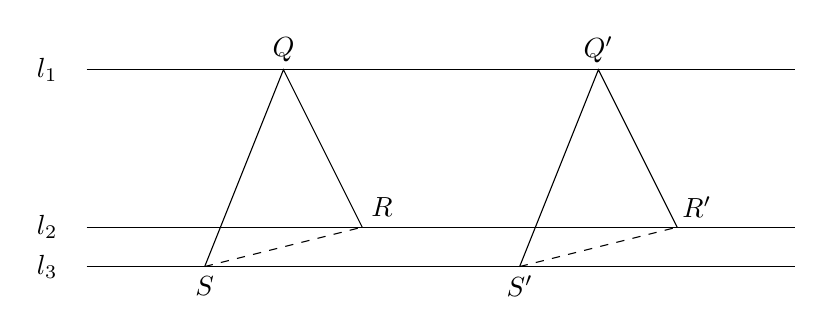
\begin{tikzpicture}
  \draw (0.5,0.5) -- (9.5,0.5);
  \draw (0.5,1) -- (9.5,1);
  \draw (0.5,3) -- (9.5,3);
  \draw[dashed] (2,0.5) -- (4,1);
  \draw[dashed] (6,0.5) -- (8,1);
  \draw (2,0.5) -- (3,3) -- (4,1);
  \draw (6,0.5) -- (7,3) -- (8,1);
  \draw (0,3) node {$l_1$};
  \draw (0,1) node {$l_2$};
  \draw (0,0.5) node {$l_3$};
  \draw (2,0.25) node {$S$};
  \draw (4.25,1.25) node {$R$};
  \draw (3,3.25) node {$Q$};
  \draw (6, 0.25) node {$S'$};
  \draw (8.25,1.25) node {$R'$};
  \draw (7,3.25) node {$Q'$};
 \end{tikzpicture}
\end{center}

\begin{center}
    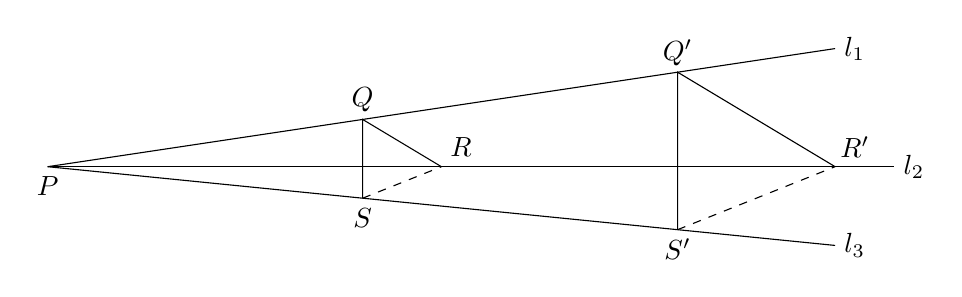
\begin{tikzpicture}
        \draw (0,0) -- (10.75,0);
        \draw (0,0) -- (10,-1);
        \draw (0,0) -- (10,1.5);
        \draw (4,-0.4) -- (4,0.6) -- (5,0);
        \draw (8,-0.8) -- (8,1.2) -- (10,0);
        \draw[dashed] (4,-0.4) -- (5,0);
        \draw[dashed] (8,-0.8) -- (10,0);
        \draw (11,0) node {$l_2$};
        \draw (10.25,-1) node {$l_3$};
        \draw (10.25,1.5) node {$l_1$};
        \draw (4,-0.65) node {$S$};
        \draw (5.25,0.25) node {$R$};
        \draw (4,0.85) node {$Q$};
        \draw (8,-1.05) node {$S'$};
        \draw (10.25,0.25) node {$R'$};
        \draw (8,1.45) node {$Q'$};
        \draw (0,-0.25) node {$P$};
    \end{tikzpicture}
\end{center}

Let us discuss some trivial cases, 
\begin{itemize}
    \item If $Q'=Q,$ then $Q+R=Q'+R'$ and since $R \ic l_2, \ R' \ic l_2$ and $R \ic Q+R,$  hence $R=R'$ is uniquely determined. Hence, it follows that $S=S'.$
    \item If $Q, \ R, \ S \in \pt$ are collinear, hence the images $Q', \ R', \ S'$ are also collinear.
\end{itemize}

Now, we will refer to the case when the lines $l_1, \ l_2, \ l_3$ are parallel as $\mathbf{D_a},$ and the case when the lines $l_1, \ l_2, \ l_3$ meet at point $P$ as $\mathbf{DP}.$

\begin{theorem}
    Axiom 4a implies $\mathbf{D_a}$ and axiom 4b P implies $\mathbf{DP}.$
\end{theorem}

\begin{proof}
    To prove $\mathbf{D_a}$, let $\tau$ be a translation which maps $Q$ to $Q'.$ By definition, $Q'+R' \parallel Q+R \parallel \tau Q + \tau R = Q' + \tau R.$ Therefore $Q'+ R' = Q'+\tau R.$ Since $l_2 \parallel Q+Q',$ hence $l_2 \in \zeta_\tau$ and $\tau R \ic l_2.$ Therefore $\tau R= R'.$ Similarly, we get $\tau S = S'.$ And therefore, $R+S \parallel \tau R + \tau S \parallel R'+S'. $ \\
    To prove $\mathbf{DP}$, let $\sigma$ be a dilatation which fixes $P$ and maps $Q$ to $Q'.$ By definition, $Q'+R' \parallel Q+R \parallel \sigma Q + \sigma R = Q' + \sigma R.$ Therefore $Q'+ R' = Q'+\sigma R.$ Since $l_2 = P+R,$ hence $l_2 \in \zeta_\sigma$ and $\sigma R \ic l_2.$ Therefore $\sigma R= R'.$ Similarly, we get $\sigma S = S'.$ And therefore, $R+S \parallel \sigma R + \sigma S \parallel R'+S'. $    
\end{proof}

\begin{theorem}
    $\mathbf{D_a}$ implies axiom 4a and $\mathbf{DP}$ axiom 4b P. 
\end{theorem}

\begin{proof}
    Suppose each line contains only two points. Then by theorem 2, there are two lines in a given pencil of parallel lines. Hence only four points exists in a given pencil, and hence in our geometry. This resembles the smallest geometry that we know in which first three axioms hold, $\Z_2^2.$ Let the four points of the geometry be $A, \ B, \ C, \ D$. Hence, there are six lines $A+B, \ A+C, \ A + D, \ B+C, \ B+D, \ C +D$. This geometry holds all axioms, especially axioms 4a and 4b. Therefore we now assume that each line contains at least three points and that for any given two lines, there exists a point such that it doesn't lie on either of the lines. \\ 
    Assume $\mathbf{D_a},$ let any $Q, \ Q' \in \pt$ and $Q \neq Q'.$ Let us associate a map $\eta_Q$ which maps $Q$ to $Q'$ and is only defined for any $R \in \pt$ such that $(R,Q+Q') \not \in \ic.$ Let $l \in \li, \ l \parallel Q+Q'$ and $R\ic l,$ then $l \neq Q+Q'.$ Let $m \in \li, \ m \parallel Q+R$ and $Q' \ic m,$ then $m \neq Q+R.$ Since $Q+Q' \not \parallel Q+R,$ hence $l \not \parallel m.$ Let $R' \in \pt$ such that $R' \ic l$ and $R' \ic m.$ Hence, $R' \neq Q'$ and $R' \neq R.$ The construction in simpler terms, $R+R' \parallel Q+Q'$ and $Q+R \parallel Q' + R',$ these explain the image $R'$ of $R$ and the map $\eta_Q.$

    \begin{center}
     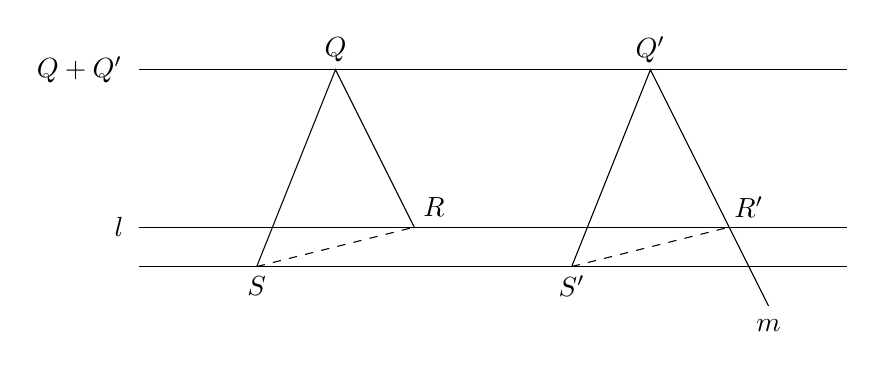
\begin{tikzpicture}
      \draw (0.5,0.5) -- (9.5,0.5);
      \draw (0.5,1) -- (9.5,1);
      \draw (0.5,3) -- (9.5,3);
      \draw[dashed] (2,0.5) -- (4,1);
      \draw[dashed] (6,0.5) -- (8,1);
      \draw (2,0.5) -- (3,3) -- (4,1);
      \draw (6,0.5) -- (7,3) -- (8.5,0);
      \draw (-0.25,3) node {$Q+Q'$};
      \draw (0.25,1) node {$l$};
      \draw (8.5,-0.25) node {$m$};
      \draw (2,0.25) node {$S$};
      \draw (4.25,1.25) node {$R$};
      \draw (3,3.25) node {$Q$};
      \draw (6, 0.25) node {$S'$};
      \draw (8.25,1.25) node {$R'$};
      \draw (7,3.25) node {$Q'$};
     \end{tikzpicture}
    \end{center}

    Since we have $R, \ R',$ we can now construct a map $\eta_R,$ which maps $R$ to $R'.$ With the same construction, it will also send $Q$ to $Q'.$ Hence the same way, let us find the image of any $S \in \pt$ such that $(S, R+R') \not \in \ic,$ and $(S, Q+Q') \not \in \ic.$ Hence $S+S' \parallel Q+Q' \parallel R+R', \ Q+R \parallel Q'+R',$ and $Q+S \parallel Q'+S'.$  Hence we can uniquely determine the image $S'$ using the map $\eta_Q.$ Hence by $\mathbf{D_a},$ $R+S \parallel  R'+S'.$ Since $S+S' \parallel R+R'$ and $R+S \parallel  R'+S',$ hence $S'$ is also an image under the map $\eta_R$. Hence we can clearly see that the map $\eta_Q, \ \eta_R$ agree on the any $S \in \pt$ such that $(S, R+R') \not \in \ic,$ and $(S, Q+Q') \not \in \ic.$ Now, as we have $S, \ S'$, we can now construct a map $\eta_S,$ which maps $S$ to $S'.$ With the same construction, it will also send $Q$ to $Q'$ and $R$ to $R'.$ Hence, we know that $\eta_Q, \ \eta_R, \  \eta_S$ agree on the any $T \in \pt$ such that $(T, S+S') \not \in \ic,$ $(T, R+R') \not \in \ic,$ and $(T, Q+Q') \not \in \ic.$ Now, the desired map $\tau$ is the combination of the three maps: for any point $T$ the image shall be the image under one of the three maps (for whichever it is defined) . This map $\tau$ has the property that $\tau(Q ) = Q$'. \\
    
    Now, we need to show that $\tau$ is a dilatation .  Let any $U, \ V \in \pt,$ and one of the lines $Q+Q',$ $R+R'$ or $S+S'$ will not contain $U, V.$ Without loss of generality, let us assume that $Q+Q'$ is such a line, that is $(U,Q+Q') \not \in \ic$ and $(V, Q+Q') \not \in \ic.$ Hence, we will use the map $\eta_Q$ to determine the image of $U, \ V.$ For $U+V \parallel Q+Q',$ then $U'\ic U+V $ and $ V' \ic U+V $, then  $U'+V'=U+V.$ For $U+V \not \parallel Q+Q',$ then using the same construction as we did to find the images of $R$ and $S,$ and proved that $R+S \parallel R'+S'$, and hence the same way, we can find the images of $U$ and $V,$ and we can prove that $U+V \parallel U'+V'.$ Hence, $\tau$ is a dilatation, and therefore a translation as all the traces are a pencil of parallel lines. \\

    Assume $\mathbf{DP},$ let any $P, \ Q, \ Q' \in \pt$ and all the points are distinct and collinear. Let us associate a map $\nu_Q$ which fixes P and maps $Q$ to $Q'$ and is only defined for any $R \in \pt$ such that $(R,Q+Q') \not \in \ic.$ 
    Let $l \in \li, \ l =P+R$, then $l \neq Q+Q'.$ Let $m \in \li, \ m \parallel Q+R$ and $Q' \ic m,$ then $m \neq Q+R.$ Since $P+R \not \parallel Q+R,$ hence $l \not \parallel m.$ Let $R' \in \pt$ such that $R' \ic l$ and $R' \ic m.$ Hence, $R' \neq Q'$ and $R' \neq R.$ The construction in simpler terms, $P \ic R+R'$ and $Q+R \parallel Q' + R',$ these explain the image $R'$ of $R$ and the map $\eta_Q.$

    \begin{center}
        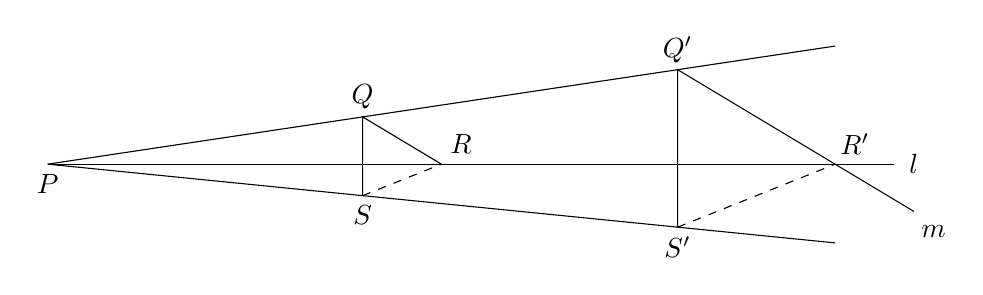
\begin{tikzpicture}
            \draw (0,0) -- (10.75,0);
            \draw (0,0) -- (10,-1);
            \draw (0,0) -- (10,1.5);
            \draw (4,-0.4) -- (4,0.6) -- (5,0);
            \draw (8,-0.8) -- (8,1.2) -- (11,-0.6);
            \draw[dashed] (4,-0.4) -- (5,0);
            \draw[dashed] (8,-0.8) -- (10,0);
            \draw (11,0) node {$l$};
            \draw (11.25,-0.85) node {$m$};
            \draw (4,-0.65) node {$S$};
            \draw (5.25,0.25) node {$R$};
            \draw (4,0.85) node {$Q$};
            \draw (8,-1.05) node {$S'$};
            \draw (10.25,0.25) node {$R'$};
            \draw (8,1.45) node {$Q'$};
            \draw (0,-0.25) node {$P$};
        \end{tikzpicture}
    \end{center}

    Since we have $R, \ R',$ we can now construct a map $\nu_R,$ which maps $R$ to $R'.$ With the same construction, it will also send $Q$ to $Q'.$ Hence the same way, let us find the image of any $S \in \pt$ such that $(S, R+R') \not \in \ic,$ and $(S, Q+Q') \not \in \ic.$ Hence $(P, Q+Q'), (P,R+R'), (P,S+S') \in \ic,  \ Q+R \parallel Q'+R',$ and $Q+S \parallel Q'+S'.$  Hence we can uniquely determine the image $S'$ using the map $\nu_Q.$ Hence by $\mathbf{DP},$ $R+S \parallel  R'+S'.$ Since $P\ic S+S'$ and $R+S \parallel  R'+S',$ hence $S'$ is also an image under the map $\nu_R$. Hence we can clearly see that the map $\nu_Q, \ \nu_R$ agree on the any $S \in \pt$ such that $(S, R+R') \not \in \ic,$ and $(S, Q+Q') \not \in \ic.$ Now, as we have $S, \ S'$, we can now construct a map $\nu_S,$ which maps $S$ to $S'.$ With the same construction, it will also send $Q$ to $Q'$ and $R$ to $R'.$ Hence, we know that $\nu_Q, \ \nu_R, \  \nu_S$ agree on the any $T \in \pt$ such that $(T, S+S') \not \in \ic,$ $(T, R+R') \not \in \ic,$ and $(T, Q+Q') \not \in \ic.$ Now, the desired map $\sigma$ is the combination of the three maps: for any point $T$ the image shall be the image under one of the three maps (for whichever it is defined) . This map $\sigma$ has the property that $\sigma(Q ) = Q$'. \\
    
    Now, we need to show that $\sigma$ is a dilatation .  Let any $U, \ V \in \pt,$ and one of the lines $Q+Q',$ $R+R'$ or $S+S'$ will not contain $U, V.$ Without loss of generality, let us assume that $Q+Q'$ is such a line, that is $(U,Q+Q') \not \in \ic$ and $(V, Q+Q') \not \in \ic.$ Hence, we will use the map $\nu_Q$ to determine the image of $U, \ V.$ For $(P, U+V) \in \ic,$ then $U'\ic U+V $ and $ V' \ic U+V $, then  $U'+V'=U+V.$ For $(P, U+V) \not \in \ic,$ then using the same construction as we did to find the images of $R$ and $S,$ and proved that $R+S \parallel R'+S'$, and hence the same way, we can find the images of $U$ and $V,$ and we can prove that $U+V \parallel U'+V'.$ Hence $\sigma$ is the desired dilatation. \\
    
\end{proof}

In the light of theorem 13 and theorem 14, Desargues' Theorem is another geometric interpretation of the axioms 4a and 4b P.
\end{document}
